\section{Background} \label{sec:background}

In this section, we provide background on the application of deep
learning in robotics, particulary autonomous vehicles.

\subsection{Deep End-to-End Learning in Autonomous Vehicles}

%% - explosion of AI
%% - in particular, application of DNN in perception and control of robotics systems.
%% - end-to-end control is a promising technique.
%%   levine's publications?
%% - examples: nvidia's DAVE-II prototype, forest navigating drone
%% challenge problem: computing at low cost?

To solve the problem of autonomous driving, a standard approach has
been decomposing the problem into multiple sub-problems,
such as lane marking detection, path planning, and low-level
control, which together form a processing pipeline~\cite{Bojarski2016}.
Recently, researchers are exploring another approach that dramatically
simplifies the standard control pipeline by applying deep neural
networks to directly produce control outputs from senor
inputs~\cite{Levine2016}. Figure~\ref{fig:end-to-end-control}
shows the differences between two two approaches.

\begin{figure}[h]
  \centering
  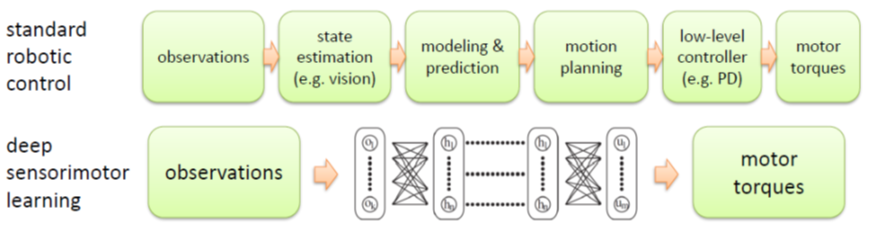
\includegraphics[width=.5\textwidth]{figs/endtoend}
  \caption{Standard robotics control vs. DNN based end-to-end
    control. \fixme{figure must be redrawn}}
  \label{fig:end-to-end-control}
\end{figure}

The use of neural networks for end-to-end control of autonomous
driving was first demonstrated in late 1980s~\cite{Pomerleau1989}, but
its success has been limited at the time as its performance was not
sufficient enough. 

%% \cite{Levine2016}: ``In this paper, we aim to answer
%% the following question: does training the perception and control systems jointly end-toend
%% provide better performance than training each component separately?''

%% \cite{Bojarski2016} nvidia paper
%% ``We trained a convolutional neural network (CNN) to map raw pixels from
%% a sin- gle front-facing camera directly to steering commands.''

%% ``Compared to explicit decomposition of the problem, such as lane
%% marking detec- tion, path planning, and control, our end-to-end system
%% optimizes all processing steps simultaneously. We''

%% UPenn's f1/10 BOM: $3,628.37	
%% http://f1tenth.org/
%% http://selfdrivingcars.mit.edu/
%% http://fast.scripts.mit.edu/racecar/
%% https://github.com/mit-racecar
%% https://mit-racecar.github.io/

\subsection{Embedded Multicore Single-Board-Computers}

- computing has been a obstacle.
- performance, but also constraints size, weight, and power as well as
cost senstive nature of industries including automtive.
- many new embeded computing platforms emerged: affordable and
powerful. raspberry pi, nvidia's embedded platforms tout their
superiority in GPU based acceleration of the AI tasks.

Our primary objective of this study are
- to understand the necessary computing performance for applying AI
technology based robotics systems, and 
- what kind of computing architecture and runtime supports
are most appropriate for such workload.

Toward to achieve the two goals, we implement a low-cost autonomous
car platform as a case study, as we will explain in the following
section. 
